\documentclass[letterpaper,11pt]{article}
\oddsidemargin -1.0cm \textwidth 17.4cm

\usepackage[utf8]{inputenc}
\usepackage[activeacute,spanish]{babel}
\usepackage{amsfonts,setspace}
\usepackage{amsmath}
\usepackage{amssymb, amsmath, amsthm}
\usepackage{comment}
\usepackage{amssymb}
\usepackage{dsfont}
\usepackage{anysize}
\usepackage{multicol}
\usepackage{enumerate}
\usepackage{graphicx}
\usepackage[left=2cm,top=2cm,right=2cm, bottom=2cm]{geometry}
\setlength\headheight{2em} 
\usepackage{fancyhdr}
\pagestyle{fancy}
\fancyhf{}


\renewcommand{\labelenumi}{\normalsize\bfseries P\arabic{enumi}.}
\renewcommand{\labelenumii}{\normalsize\bfseries (\alph{enumii})}
\renewcommand{\labelenumiii}{\normalsize\bfseries \roman{enumiii})}


\DeclareMathOperator{\sen}{sen}
\DeclareMathOperator{\senh}{senh}
\DeclareMathOperator{\arcsen}{arcsen}
\DeclareMathOperator{\tg}{tg}
\DeclareMathOperator{\arctg}{arctg}
\DeclareMathOperator{\ctg}{ctg}
\DeclareMathOperator{\dom}{Dom}
\DeclareMathOperator{\sech}{sech}
\DeclareMathOperator{\rec}{Rec}
\DeclareMathOperator{\inte}{Int}
\DeclareMathOperator{\adh}{Adh}
\DeclareMathOperator{\fr}{Fr}
\DeclareMathOperator{\Ima}{Im}
\DeclareMathOperator{\dist}{dist}
\DeclareMathOperator{\argmin}{\text{argmín}}
\let\lim=\undefined\DeclareMathOperator*{\lim}{\text{lím}}
\let\max=\undefined\DeclareMathOperator*{\max}{\text{máx}}
\let\min=\undefined\DeclareMathOperator*{\min}{\text{mín}}
\let\inf=\undefined\DeclareMathOperator*{\inf}{\text{ínf}}


\newcommand{\pint}[2]{\left< #1,#2\right>}
\newcommand{\ssi}{\Longleftrightarrow}
\newcommand{\imp}{\Longrightarrow}
\newcommand{\pmi}{\Longleftarrow}
\newcommand{\ipartial}[2]{\dfrac{\partial #1}{\partial #2}}
\newcommand{\ider}[2]{\dfrac{d #1}{d #2}}
\newcommand{\iipartial}[2]{\dfrac{\partial^2 #1}{\partial #2^2}}
\newcommand{\iider}[2]{\dfrac{d^2 #1}{d #2^2}}
\newcommand{\ijpartial}[3]{\dfrac{\partial^2 #1}{\partial #2 \partial #3}}
\newcommand{\N}{\mathbb{N}}
\newcommand{\Z}{\mathbb{Z}}
\newcommand{\C}{\mathbb{C}}
\newcommand{\Q}{\mathbb{Q}}
\newcommand{\R}{\mathbb{R}}
\newcommand{\K}{\mathbb{K}}
\newcommand{\sol}{\textbf{\emph{Soluci\'on: }}}
\newcommand{\dem}{\textbf{\emph{Demostraci\'on: }}}
\newcommand{\aux}[4]{\Large \textbf{Clase Auxiliar N#1: #2}}
\newcommand{\pauta}[4]{\Large \textbf{Pauta #1 N#2}}
\newcommand{\enc}[3]{\Large \textbf{#1}}
\newcommand{\norm}[1]{\lVert #1\rVert }
\newcommand{\vabs}[1]{\lvert #1\rvert}

\begin{document}

\fancyhead[L]{\itshape{Facultad de Ciencias F\'isicas y Matem\'aticas}}
\fancyhead[R]{\itshape{Universidad de Chile}}

\begin{minipage}{11.5 cm}
\begin{flushleft}
\hspace*{-0.6cm}\textbf{MA2001-4 Cálculo en Varias Variables}\\
\hspace*{-0.6cm}\textbf{Profesor:} Javier Ramírez G.\\
\hspace*{-0.6cm}\textbf{Auxiliar:} Alejandro Silva C.\\

\end{flushleft}
\end{minipage}

\begin{picture}(2,3)
    \put(370,-4){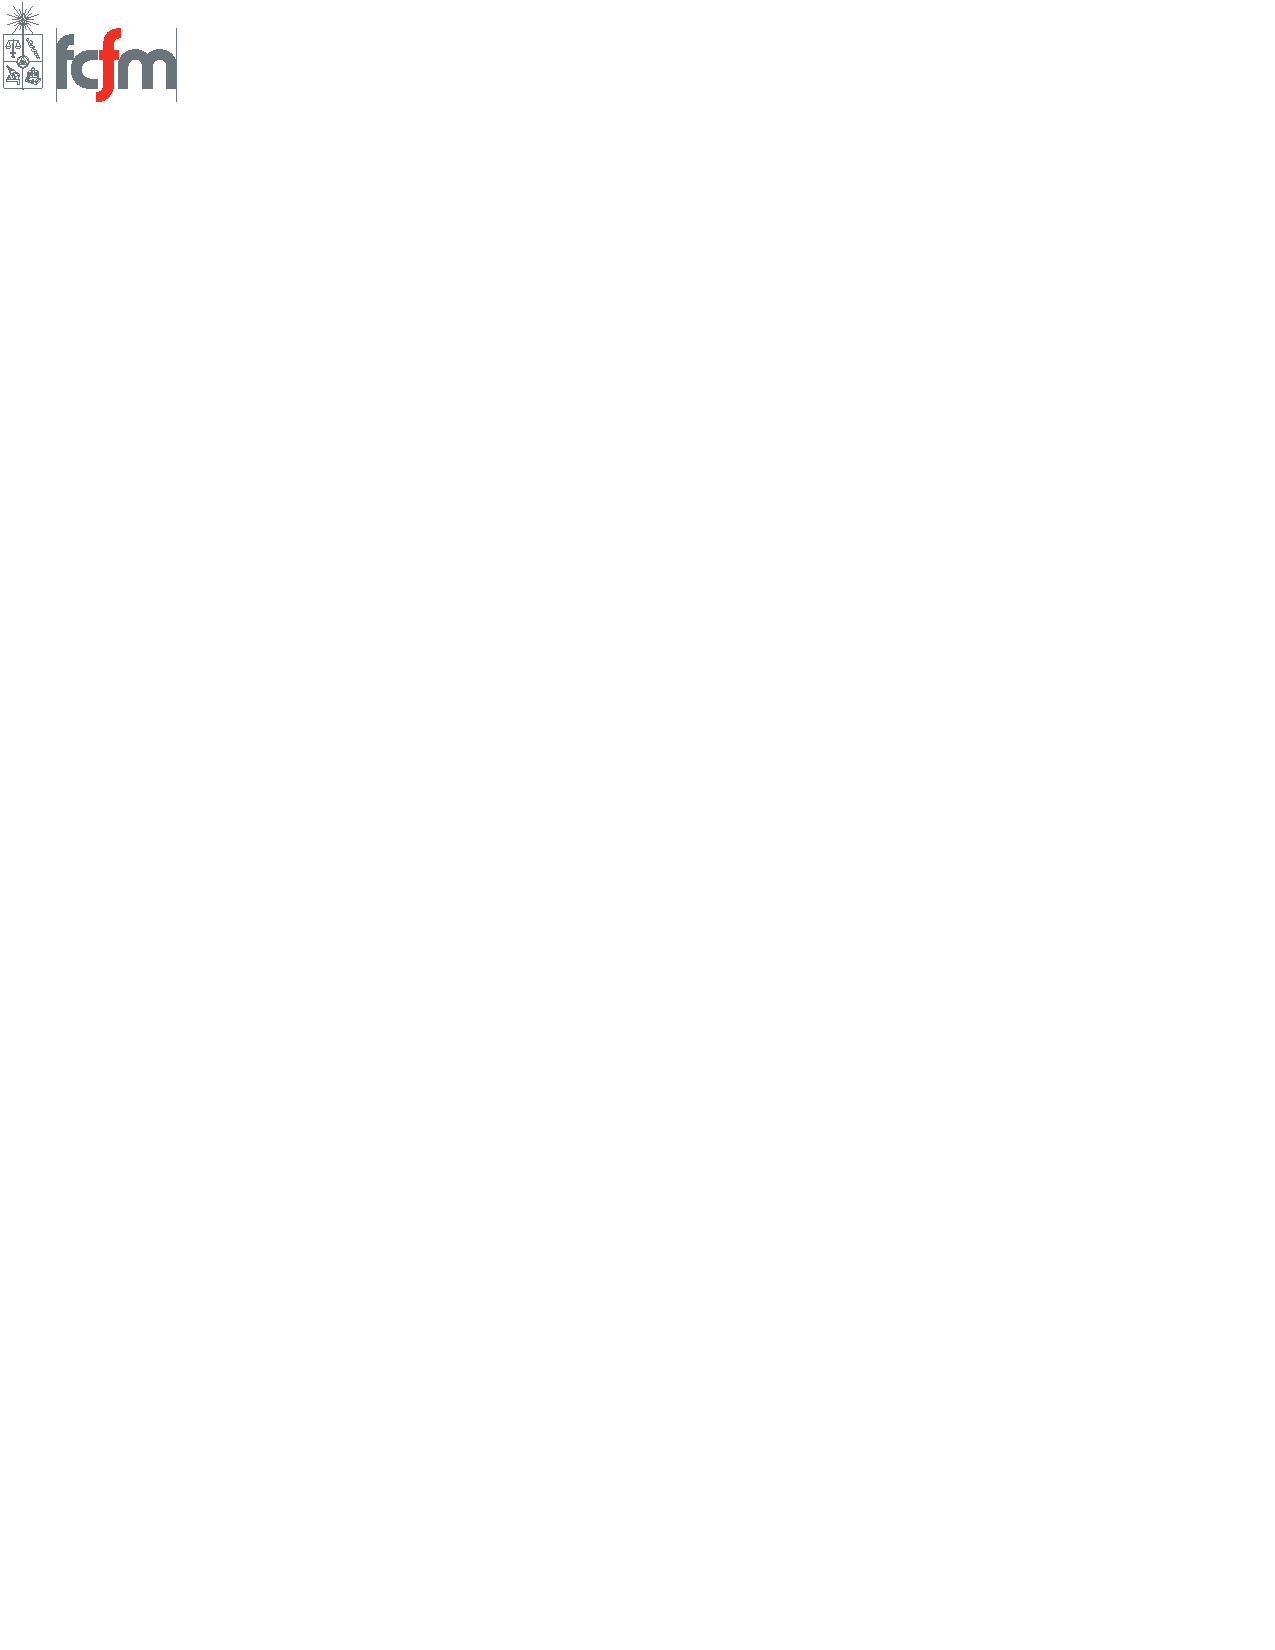
\includegraphics[scale=1.2]{fcfm2.pdf}}
\end{picture}

\begin{center}
	\LARGE \bf{Auxiliar \#1}\\
\end{center}

\vspace{-1cm}
\begin{enumerate}\setlength{\itemsep}{0.4cm}	
\item[]


\item \textbf{(Coordinada)} Consideremos $\mathcal{M}_{d\times d}(\R)$ el espacio de las matrices cuadradas de $d\times d$. Definimos

%%%%%%% Opción 1 (Norma de operador o inducida)
\begin{align*}
\norm{\cdot} : \mathcal{M}_{d\times d}(\R)&\to\R\\
A & \mapsto \sup_{\substack{x\in\R^d :\\
                  \norm{x}_1=1}}\norm{Ax}_1
\end{align*}



\begin{enumerate}

%%%%%%%% Opción 2 (Norma 1 matricial)
% \begin{align*}
% \norm{\cdot}_{\mathcal{M}} : \mathcal{M}_{n\times n}(\R)&\to\R\\
% A & \mapsto \max_{j=1,...,n}\left(\sum_{i=1}^n\vabs{a_{ij}}\right)
% \end{align*}




\item Muestre que $\norm{\cdot}$ es una norma en $\mathcal{M}_{d\times d}$.
\item Muestre que para toda matriz $A\in\mathcal{M}_{d\times d}$ y para todo vector $x\in \R^d$ se cumple que:
\[\norm{Ax}_{1}\leq \norm{A}\norm{x}_1\]
\item Pruebe que para todo par de matrices $A,B\in\mathcal{M}_{d \times d}$ se tiene que
\[\norm{A\cdot B}\leq \norm{A}\norm{B}\]
\end{enumerate}	

\item Considere $E$ un espacio vectorial normado cualquiera.
\begin{enumerate}
    \item Pruebe que $\phi, E$ son conjuntos abiertos.
    \item Pruebe que si $\{A_i\}_{i\in I}\subseteq E$ es una familia de abiertos, con $I$ una familia de índices cualquiera , entonces el conjunto
    \[\bigcup_{i\in I}A_i\]
    también es abierto.
    \item Pruebe que si $\{A_i\}_{i=1}^n\subseteq E$ es una familia finita de abiertos, entonces el conjunto
    \[\bigcap_{i=1}^nA_i\]
    también es abierto.
\end{enumerate}

\item Estudie la convergencia de la sucesión $(x_n,y_n)_{n\in\N}\subseteq \R^2$, dada por:
\[(x_n,y_n):=\bigg(\frac{2n^2+(-1)^n}{3n^2},ne^{-n}\sen\bigg(\frac{1}{n}\bigg)\bigg).\]



\end{enumerate}	
\end{document}